\section{Simulation}
Zur Überprüfung der Implementierung wurde die Bewegung des Crawlers zunächst simuliert. Die Simulation bietet ein Ground Truth ohne aufwändiges Kameratracking vorteilhaft, sowie verschiedene Karten. Diese können als beliebige konvexe Polygone definiert werden, in denen sich der Crawler frei bewegen kann.
Um Komponenten der Simulation zur Auswertung des Experiments wiederverwenden zu können, wurde auf einen modularen Aufbau geachtet. Die grobe Struktur des Frameworks wird in \ref{fig:class} verdeutlicht. Es gibt eine einheitliche Schnittstelle, die zur Kommunikation mit der realen Crawler-Hardware, sowie dem simuliertem Crawler genutzt wird. Die Steuerung ist über drei verschiedene Modi möglich:
\begin{itemize}
	\item Auswahl der Bewegungsanweisungen durch den Benutzer
	\item Zufällige Bewegungsanweisungen
	\item Wiedergabe eines aufgezeichneten Bewegungspfads des echten Crawlers
\end{itemize}

\begin{figure}
	\centering
	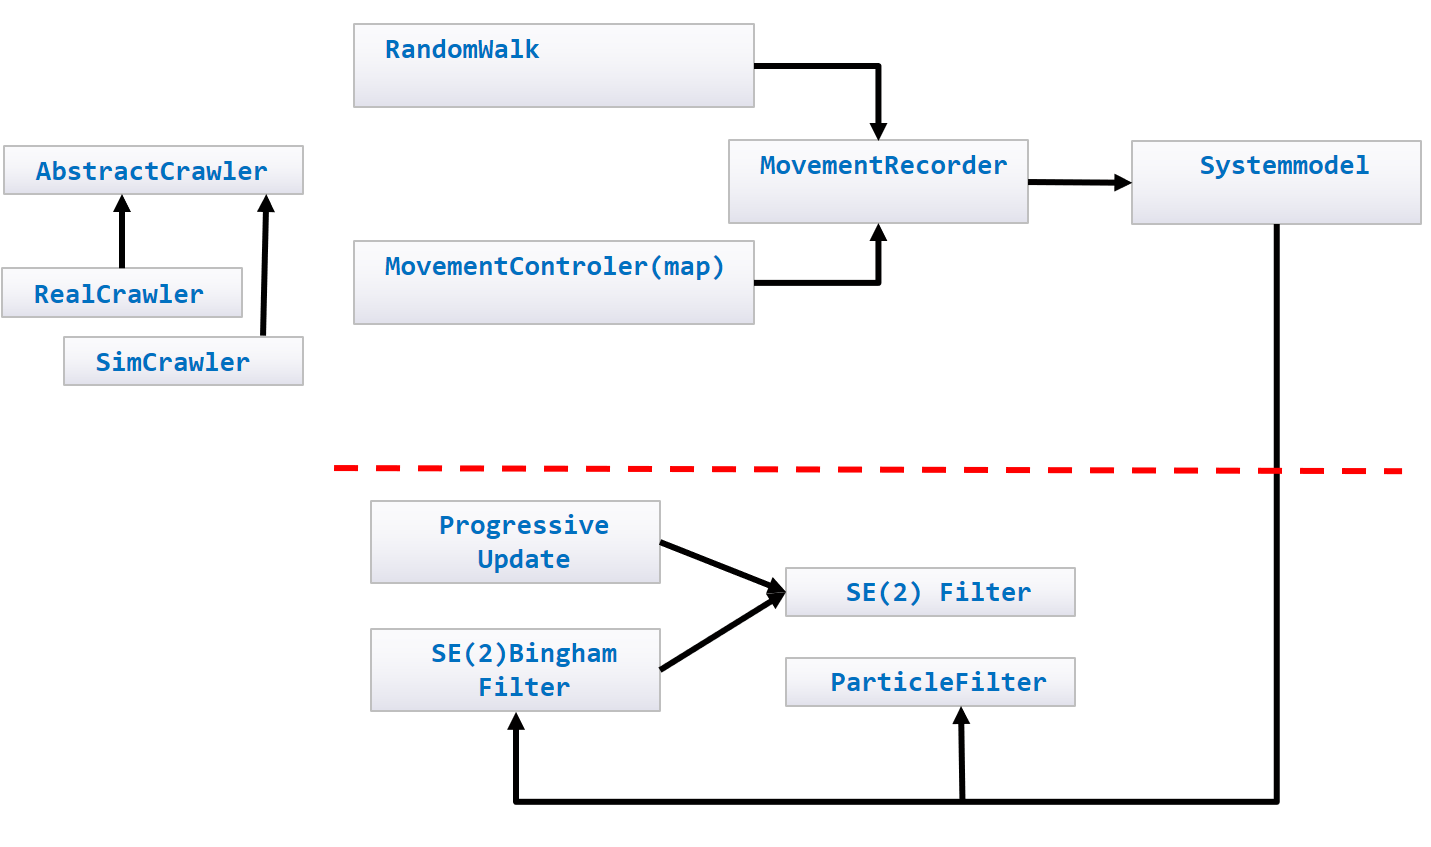
\includegraphics[width=0.9\linewidth]{Images/class.png}  
	\caption{Aufbau des Simulationsframeworks}
	\label{fig:class}
\end{figure}

Crawler Modell
Das vereinfachte Modell des Crawlers, das zur Simulation verwendet wurde ist in \ref{fig:ModelCrawler} zu sehen. Der Ursprung des Koordinatensystems liegt auf der vorderen roten LED, die zum Tracking der Position verwendet wurde. Der eigentlich kegelförmige Messbereich der vier Ultraschallsensoren wurde als Halbgerade modelliert.

\begin{figure}[ht]
	\centering
	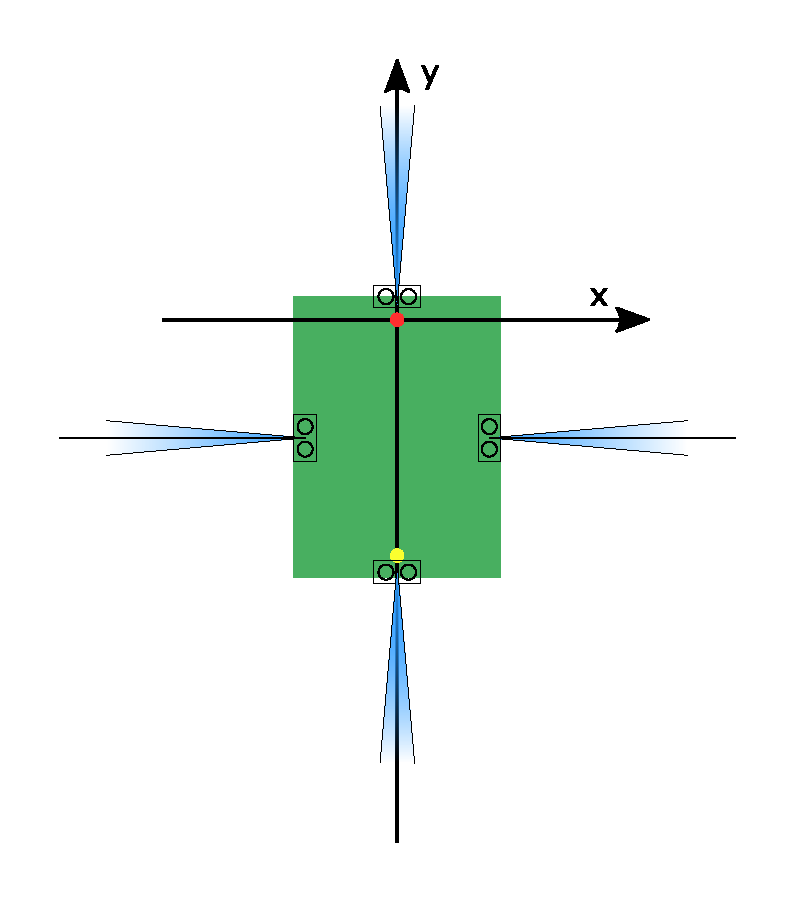
\includegraphics[]{Images/ModelCrawler}  
	\caption{In der Simulation verwendetes Schema des Crawlers mit lokalem Koordinatensystem. Markeirt sind die vier Ultraschallsensoren mit Messbereich, sowie die zwei verschiedenfarbenen LEDs.}
	\label{fig:ModelCrawler}
\end{figure}

\subsection{Systemmodell}
Vorwissen über das System findet im Systemmodell Anwendung. Mit der Überführungsfunktion $a$ wird der Folgezustand $\vec{x}_{t+1}$ aus dem aktuellem Zustand $\vec{x}_t$ abgeleitet. Der verwendete Zustandsraum $\mathbb{S} \times \IR^2$ beschreibt die position und Orientierung des Crawlers.


\begin{align*}
\vec{x}_{t+1} = a(\vec{x}_t) \oplus w_t
\end{align*}

Die Folge von Bewegungsbefehlen an den Crawler ist bekannt. Je nach Bewegungsbefehl ist die entsprechende Überführungsfunktion zu wählen:

\begin{equation}
    a(\vec{x}_t, command) = 
        \begin{cases}
            a_{fwd} \oplus w_{fwd},& \text{falls } command= fwd \\
            a_{left} \oplus w_{left},& \text{falls } command= left\\
            a_{right} \oplus w_{right},& \text{falls } comman= right
        \end{cases}
\end{equation}

Die tatsächliche ausgeführten Schritte variieren jedoch, auch für gleichbleibende Bewegungsrichtungen. Dies wir in Abbildung \ref{fig:moves} deutlich. Deswegen wird bei jedem Schritt zusätzlich ein Rauschterm $w_t$ addiert. Dies lässt sich in SE(2) durch die Multiplikation der dualen Quaternionen darstellen, was durch den $\oplus$-Operator ausgedrückt wird.
Die Schrittlängen und Drehungen wurden in einem Vorexperiment durch Tracking der LEDs mit der Deckenkamera aufgenommen. Es wurden drei SE(2)-Bingham-Verteilungen auf die gewonnen Daten angepasst, aus denen die jeweiligen $w_t$ zufällig gezogen werden.





\begin{figure}[ht]
	\centering
    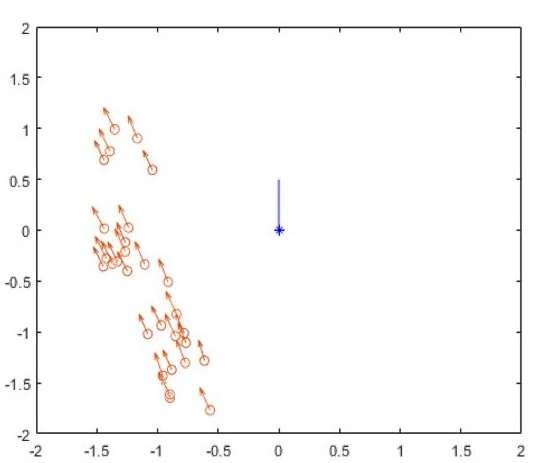
\includegraphics[width=.32\textwidth]{Images/links.jpg}
    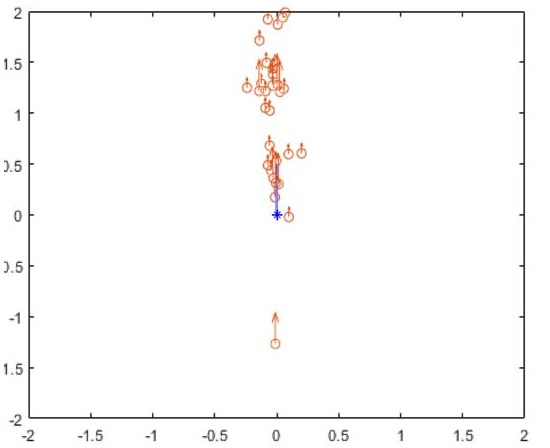
\includegraphics[width=.32\textwidth]{Images/vorne.jpg}
    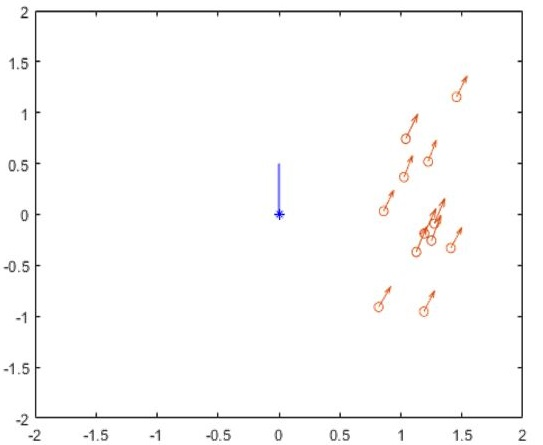
\includegraphics[width=.32\textwidth]{Images/rechts.jpg}
	\caption{Gemessene Verteilungen der Position und Rotation des Laufrobotters nach der Ausführung einer Bewegung. Blau ist der Ausgangszustand dargestellt. Die Zustände nach je einem Schritt in rot. Jede Verteilung wurde für einen der drei Bewegungsbefehle 'links', 'vorwärts' und 'rechts' mit einer Deckenkamera gemessen.}
	\label{fig:moves}
\end{figure}

Daraus werden die Erwartungswert und Varianz berechnet,und wir bezeichnen diese Datensätze als die echte Systemrauschen von Roboter.

\subsection{Messmodell}

Der Crawler kann seine momentane Position und Ausrichtung nicht direkt messen. Es stehen jediglich vier nach vorne, hinten, links und rechts gerichtet Ultraschallsensoren zur Verfügung, die Abstandsmessungen zu den nächstliegenden Wänden vornehmen könne. Die Messwerte hängen bei einer festen Karte von der Position und Ausrichtung des Crawlers ab. 
Mit dem Messmodel wird beschrieben, welche Messergebnisse bei einem Systemzustand zu erwarten sind. Eine Messung ist Abbildung vom dreidimensionalen Zustandsraum des Laufroboters $\mathbb{S} \times \IR^2$ in einen vierdimensionalen Messraum ${\IR^+}^4$.

Da die Ultraschallsensoren des Crawler nur grobe Abstandsmessungen ermöglichen, wird ein normalverteiltes mittelwertfreies Rauschen $w_t \sim \mathcal{N}(0,\sigma)$ addiert:

\begin{align*}
\vec{z}_{t} = h(\vec{x}_t) \oplus w_t
\end{align*}

$h(x_t)$ für einen Zustand $x_t$ zu berechnen ist leicht. Es muss lediglich eine Messung auf einer virtuellen Karte an der von $x_t$ beschriebenen Position durchgeführt werden. In unserem Fall lässt sich $h$ jedoch nicht einfach invertieren. $h^{-1}$ muss nicht eindeutig sein. Die selbe Messung könnte kann in mehreren verschiedenen Zuständen beobachtet werden.
Aus $h$ lässt sich ohne weiteres die eine Likelihood $f(z_t | x_t)$ ableiten [3]. Diese beschreibt die Plausibilität einer Messung für einen gegebenen Zustand. Die Likelihood kann folgendermaßen berechnet werden $f(z_t | x_t) = f_{\mathcal{N}}(h(x_t)  - z_t)$, wobei  $f_{\mathcal{N}}$ komponentenweise in eine Normalverteilung $\mathcal{N}$ einsetzt und die resultierenden Wahrscheinlichkeiten multipliziert. Die Abbildung \ref{fig:likelihood} zeigt den Crawler in der Position im linken Bild, mit der Likelihood-Funktion für den gezeigten Zustand rechts. Der hell gelbe Punkt rechts, mit der größten Wahrscheinlichkeit befindet sich an der Stelle des Crawlers, von dem die Messung $z_t$ stammt.

\begin{figure}[ht]
	\centering
	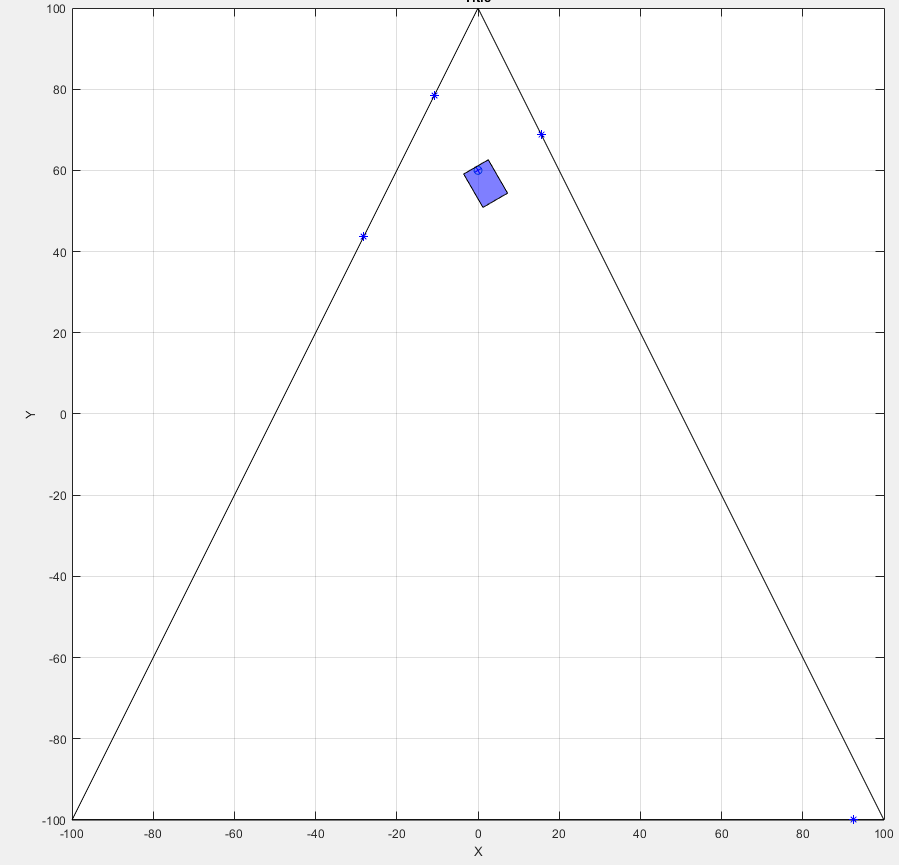
\includegraphics[width=8cm]{Images/likelihoodPosition.png}
    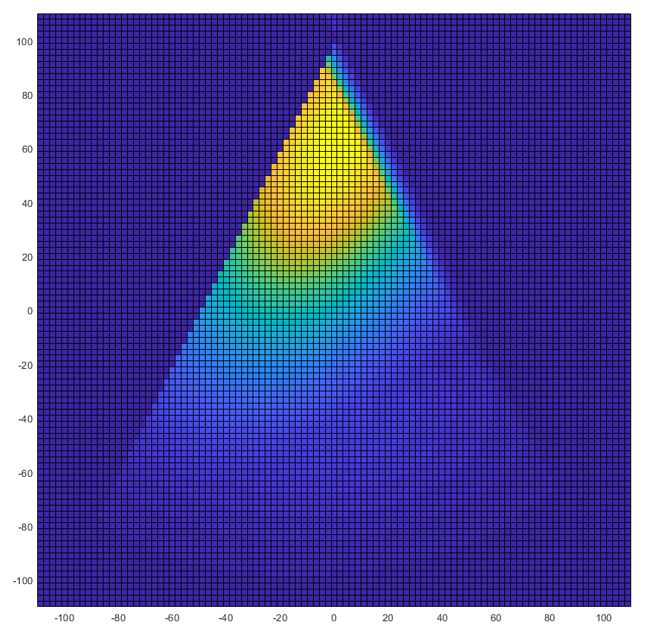
\includegraphics[width=8cm]{Images/likelihood.jpg}  
	\caption{Linkes Bild: In blau ist der Crawler auf der dreieckigen Karte eingetragen. Rechts die Likelihood-Funktion $f(z_t | x_t)$, für die Messung, die der Crawler im linken Bild aufnimmt.}
	\label{fig:likelihood}
\end{figure}

\subsection{Progressive Updates}

Nach Anwendung des Systemmodells im Prediction-Schritts folgt  der Aktualisierungsschritt, der den geschätzten Zustand $x_{t}^{e}$ durch Einbeziehung der Messung $z_{t}$ korrigiert
Beim Progressiven Update werden vom aktuell geschätze Systemzustand $x_{t}^{e}$ dazu zunächst deterministisch Proben gezogen. Anstatt diese in einem Schritt mit den Werten der Likelihood-Funktion neu zu gewichten, wird iterativ vorgegangen [4]. Dies ist nach der Regel von Bayes möglich, wenn die $\lambda_1 + \lambda_s$ eine Zerlegung der $1$ bilden. Dadurch kann eine Degenerierung der Proben mit Likelihoodwerten nahe null vermieden werden. Degenerierte Proben verringern die Genauigkeit des Filters. Außerdem ermöglicht das Progressive Update die Korrektur des geschätzten Orts ohne die Messfunktion $h$ invertieren zu müssen. Gemessene Werte können direkt in die Likelihood eingesetzt werden.

\begin{align*}
	f(\vec{x} | \vec{z}) \propto f(\vec{z} | \vec{x}) * f(\vec{x})\\
	= (f(\vec{z} | \vec{x})^{\lambda_1} * ... * f(\vec{z} | \vec{x})^{\lambda_s}) * f(\vec{x})
\end{align*}


 Durch den folgenden Ablauf wird garantiert, dass der Quotient zwischen dem kleinsten neuen Gewicht
$l_{min}$ und das größte neue Gewicht $l_{max}$ nicht über einen vorbestimmten Schwellwert steigt. Dieser Schwellwert wird mit $\tau$ bezeichnet.
\\

\begin{alogrithm}
	\caption{Ablauf des Progressiven Updates}\label{update}
	\begin{algorithmic}[1]
		\Procedure{Update}{measurement $z_t$, likelihood $f(z_t | x_t)$, predicted density $x_{t}^{e}$}
	  \State $\Lambda\leftarrow 1$
	  \State $x_{t} \leftarrow x_{t}^{e}$
	  \While{ $\Lambda>0$ }
	  \State $(s_{1},...,s_{L},\omega_{1},...,\omega_{L})\leftarrow \text{sampleDeterministicly}(x_t)$
	  \State $\omega_{min}\leftarrow min(f(z_{k}|s_{k}))$
      \State $\omega_{max}\leftarrow max(f(z_{k}|s_{k}))$
	  \State $\lambda \leftarrow min(\Lambda, \frac{log(\tau)}{log(\omega_{min}/\omega_{max})})$
	  \For{$j \leftarrow 1 \textbf{to} L$}
		\State $\omega_{k} \leftarrow \omega_{k}\cdot f(z_{k}|x_{k})^{\lambda}$
      \EndFor
	  \State $x_t \leftarrow matchBingham(s_{1},...,s_{L},\omega_{1},...,\omega_{L})$
	  \State $\Lambda\leftarrow\Lambda-\lambda$
    \EndWhile
	\EndProcedure
  \end{algorithmic}

\end{alogrithm}


